\begin{XeClass}{FileChecksum}
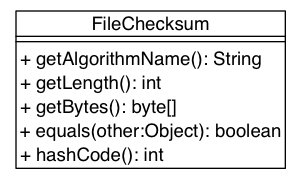
\includegraphics[width=\textwidth]{cdig/FileChecksum.png}
     
 代表文件校验和的抽象类

    \begin{XeMethod}{\XePublic \\ \XeAbstract}{String}{getAlgorithmName}
         
 校验算法名 

    \end{XeMethod}

    \begin{XeMethod}{\XePublic \\ \XeAbstract}{int}{getLength}
         
 校验和的byte长度 

    \end{XeMethod}

    \begin{XeMethod}{\XePublic \\ \XeAbstract}{byte[]}{getBytes}
         
 校验和的byte值

    \end{XeMethod}

    \begin{XeMethod}{\XePublic}{boolean}{equals}
         
 如果算法和byte值都相同,返回真值

    \end{XeMethod}

    \begin{XeMethod}{\XePublic}{int}{hashCode}
         
 返回hash值

    \end{XeMethod}

\end{XeClass}
